% CVS info. These are modified by cvs at checkout time.
% The last version of these macros found before the maketitle will be the one on the front page,
% so only the main file is tracked.
% Do not edit by hand!
% trivial test change
\RCS$Revision: 16769 $
\RCS$HeadURL: svn+ssh://svn.cern.ch/reps/tdr2/papers/EXO-10-010/tags/v1-Sep5-3pb/EXO-10-010.tex $
\RCS$Id: EXO-10-010.tex 16769 2010-09-06 21:41:01Z rharris $
%%%%%%%%%%%%% ptdr definitions %%%%%%%%%%%%%%%%%%%%%
\input{ptdr-definitions}
%%%%%%%%%%%%%%%  Title page %%%%%%%%%%%%%%%%%%%%%%%%
\cmsNoteHeader{EXO-10-001} % This is over-written in the CMS environment: useful as preprint no. for export versions
\title{Search for Dijet Resonances in 7 TeV $pp$ Collisions at CMS}% Force line breaks with \\

%Author is always "The CMS Collaboration" for PAS, so author, etc will be ignored
\address[cern]{CERN}
\address[neu]{Northeastern University}
\author[cern]{The CMS Collaboration}

% please supply the date in yyyy/mm/dd format. Today has been
% redefined to do so, but it should be fixed as of the final release date.
\date{\today}

% note that you cannot use \verb in the abstract text
\abstract{
We have used data corresponding to the integrated luminosity of 2.88 pb$^{-1}$ collected 
with the CMS experiment at the Large Hadron Collider at CERN to search for narrow resonances 
in the dijet mass spectrum. Upper limits are presented on the product of the resonance cross 
section, branching fraction into dijets, and acceptance. These generic limits are used to 
exclude at the 95\% confidence level new particles predicted 
in the following specific models: string resonances with mass less than 2.50~TeV, excited quarks with mass less than 1.58~TeV, 
and axigluons, colorons and $E_6$ diquarks in specific mass intervals, extending previously 
published limits on all models.}

% Do not comment out the following hypersetup lines (metadata). They will disappear in NODRAFT mode and are needed by CDS.
% Also: make sure that the values of the metadata items are sensible.
\hypersetup{%
pdfauthor={Dijet Group},%
pdftitle={Search for Dijet Resonances in 7 TeV $pp$ Collisions at CMS},%
pdfsubject={CMS},%
pdfkeywords={CMS, physics, software, computing}}

\maketitle %maketitle comes after all the front information has been supplied

%%%%%%%%%%%%%%%%%%%%%%%%%%%%%%%%  Begin text %%%%%%%%%%%%%%%%%%%%%%%%%%%%%

Within the Standard Model, events with two energetic jets (dijets) 
arise in proton-proton collisions from parton-parton scattering.  The
outgoing scattered partons manifest themselves as hadronic jets.  The 
dijet mass spectrum predicted by Quantum Chromodynamics (QCD) falls smoothly and steeply with 
increasing dijet mass.  Many extensions of the Standard Model predict the existence of new massive objects
that couple to quarks ($q$) and gluons ($g$), and result in resonant structures 
in the 
dijet mass spectrum.  In this letter we report a search for narrow 
resonances in the dijet mass spectrum, measured with the Compact Muon 
Solenoid (CMS) detector~\cite{refCMS} at the CERN Large Hadron Collider, at a proton-proton 
collision energy of $\sqrt{s}=7$~TeV. 

In addition to this generic search, we search for  
manifestations of eight specific models of narrow dijet resonances.
First, string resonances are Regge excitations of the quarks and gluons in string 
theory, with multiple mass-degenerate spin states and 
quantum numbers~\cite{Anchordoqui:2008di,Cullen:2000ef}. String resonances with mass
$\sim 2$ TeV decay predominantly to $qg$(91\%) with small amounts of $gg$ (5.5\%) and 
$q\bar{q}$(3.5\%).
Second, if quarks are composite
particles then excited states are expected, and we search 
for mass degenerate excited quarks  $q^*$ that decay to 
$qg$~\cite{ref_qstar}.  The compositeness scale is set to be equal to the mass of the excited quark.
Third, in a model where the symmetry group $SU(3)$ of QCD is replaced by the 
chiral symmetry $SU(3)_L\times SU(3)_R$, there are axial vector particles called
axigluons $A$, which decay to $q\bar{q}$~\cite{ref_axi}.
Fourth, the flavor-universal coloron model also embeds the $SU(3)$ of QCD in 
a larger gauge group, and predicts the presence of a color-octet coloron $C$,
which decays to $q\bar{q}$~\cite{ref_coloron}.
Fifth, grand unified theory based on the $E_6$ gauge group predicts the presence 
of scalar diquarks $D$ and $D^c$, which decay to $\bar{q}\bar{q}$ and
$qq$~\cite{ref_diquark}.
Sixth, the Randall-Sundrum (RS) model of extra dimensions predicts massive 
gravitons $G$, which decay to $q\bar{q}$ and $gg$~\cite{ref_rsg}.
For the RS graviton, the value of the dimensionless coupling
$\kappa/M_{Pl}$ is set to 0.1.
Seventh and Eighth,
models that propose new gauge symmetries often predict new 
gauge bosons $W^\prime$ and $Z^\prime$, which decay to 
$q\bar{q}$~\cite{ref_gauge}.  The $W^\prime$ and $Z^\prime$ resonances
are assumed to have standard model couplings and to have fractional widths
equal to the corresponding standard model $W$ and $Z$ bosons.


A detailed description of the CMS experiment can be found 
elsewhere~\cite{refCMS}.
The CMS coordinate system has the origin at the center of the detector, 
the $z$-axis points along the direction of the counterclockwise beam, with the transverse 
plane perpendicular to the beam. We define $\phi$ to be the azimuthal 
angle, $\theta$ to be the polar angle and the pseudorapidity as 
$\eta \equiv -\ln(\tan[\theta/2])$. 
The central feature of the CMS apparatus is a superconducting solenoid, of 6 m 
internal diameter. 
Within the field volume are the silicon pixel and strip tracker, and the barrel and
endcap calorimeters ($|\eta|<3$): a crystal electromagnetic calorimeter (ECAL) and
a brass-scintillator hadronic calorimeter (HCAL).
Outside the field volume, in the forward region, there is 
an iron-quartz fiber hadronic calorimeter ($3<|\eta|<5$).
The ECAL and HCAL cells are grouped into towers, projecting radially outward from 
the origin, for triggering purposes and to facilitate the jet reconstruction.  
In the region 
$|\eta|<1.74$ these projective calorimeter towers have segmentation 
$\Delta\eta = \Delta\phi = 0.087$, and the $\eta$ and $\phi$ width 
progressively increases at higher values of $\eta$. 
The energy in the HCAL and 
ECAL within each projective tower is summed to find the calorimeter tower energy.
Towers with $|\eta|<1.3$ contain only cells from the barrel 
calorimeters, towers in the transition region $1.3<|\eta|<1.5$ contain a mixture of 
barrel and endcap cells, and towers in the region $1.5<|\eta|<3.0$ 
contain only cells from the endcap calorimeters. 

The integrated luminosity of the selected data sample used for this
analysis is $2.88 \pm 0.32$~pb$^{-1}$.  A single-jet trigger is used in the online
software-level trigger system, known as the High-Level 
Trigger~(HLT), to select an unprescaled sample of events for this analysis.
Another single-jet trigger with a lower $p_{\rm T}$ threshold with a prescaling of
events is used for the purpose of computing trigger efficiencies.
The trigger efficiency versus dijet mass for this analysis is measured from the data
and is greater than 99.5\% for dijet masses
above 220~GeV.  
%This analysis includes all 
%dijet mass data above a threshold of 220~GeV.
%The minimum dijet mass used in this analysis, 220~GeV, is the lower edge of
%one of the a priori defined bins determined by the dijet mass resolution.
%and is synchronized to a concurrent
%analysis of the dijet centrality ratio~\cite{EXO-10-002-PAS}.


Jets are reconstructed using the anti-$k_T$ algorithm~\cite{1126-6708-2008-04-063} with the distance 
parameter $R=0.7$. The reconstructed jet energy, $E$, is defined as the scalar
sum of the calorimeter tower energies inside the jet. The jet momentum, $\vec{p}$, is the corresponding vector sum 
of the energies of towers.
The $E$ and $\vec{p}$ of a reconstructed jet are corrected as a function of transverse momentum (\pt) and $\eta$ for the 
non-linearity and inhomogeneity of the calorimeter response. The jet energy corrections were determined and validated using Monte Carlo, test beam data,
and collision data~\cite{JME-10-003-PAS}.

To remove possible instrumental and non-collisional
backgrounds in the selected sample the following selections are made.
Events in the sample are
required to have a reconstructed primary vertex with $|z|<24$ cm.
Jets are required to have a minimum
of 1\% of their total energy detected in the ECAL, a minimum
multiplicity of two calorimeter cells, ECAL or HCAL, and a maximum 
of 98\% of the total energy occurring in a single photodetection device
of the hadron calorimeter readout. 
The jet identification criteria remove 0.1\% of the events passing
the pseudorapidity constraints and the dijet mass threshold.  


The dijet system is composed of the 
two jets with the highest $p_T$ in an event (leading jets), 
and the dijet mass is given by 
$m=\sqrt{(E_1 + E_2)^2 - (\vec{p}_1 + \vec{p}_2)^2}$. 
We select events with at least two jets 
and require that the pseudorapidity separation of the two leading 
jets, $\Delta\eta=\eta_1-\eta_2$, satisfies 
$|\Delta\eta|<1.3$, and also require that both jets be in the region 
$|\eta|<2.5$. These $\eta$ cuts maximize the search sensitivity for 
isotropic decays of dijet resonances in the presence of QCD background.


In Fig.~\ref{fig1} we present the inclusive dijet mass 
distribution for $pp\rightarrow$ 2 leading jets + $X$, where $X$ can be 
anything, including additional jets. 
We plot the measured differential cross section versus dijet mass in 
bins approximately equal to the dijet mass resolution. 
The data are compared to a QCD prediction from PYTHIA~\cite{refPYTHIA}, which includes a simulation of the CMS  
detector and the jet energy corrections.  
The prediction uses CTEQ6 parton distributions~\cite{refCTEQ} and a renormalization scale $\mu=\pt$. 
The data agree with the PYTHIA prediction within the systematic uncertainties of the measurement. 
To test the smoothness of our measured cross section as a function of dijet mass, we 
fit the data with the parameterization~\cite{refCDFrun2,ATLAS_search}:

\begin{equation}
\frac{{\rm d}\sigma}{{\rm d}m} = 
\frac{P_{0} (1 - m/\sqrt{s})^{P_{1}}}{(m/\sqrt{s})^{P_{2} + P_{3} ln
(m/\sqrt{s})}}\ ,
\end{equation}

with the four parameters $P_0$, $P_1$, $P_2$ and $P_3$. 
In Fig.~\ref{fig1} we show both the data and the fit, 
which has a $\chi^2$ of 32 for 31 degrees of freedom.  In Fig.~\ref{fig2} we show
the ratio between the data and the fit.  The data are well described by 
the smooth parameterization and show no evidence of new particles.

 We search for narrow resonances, for which the
natural resonance width is negligible compared to the CMS dijet mass 
resolution. In Figs.~\ref{fig1} and \ref{fig2} we show the 
predicted dijet mass distribution for string resonances (S) and excited quarks ($q$*) using the 
PYTHIA Monte Carlo~\cite{refPYTHIA} and the CMS detector simulation.
The mass resolution has a Gaussian core from 
jet energy resolution and a long tail towards low mass from QCD radiation.
 The dijet mass distribution of narrow dijet resonances depends on 
the type of partons involved in the resonance production and decay, because this affects both the 
amount of radiation and the final state jet response in
the CMS detector.
In Fig.~\ref{fig3} we show examples of the predicted dijet mass distribution of resonances from
three different parton pairings: $qq$ (or $q\bar{q}$) resonances 
from the process $G \rightarrow q\bar{q}$~\cite{ref_rsg}, 
$qg$ resonances from the process $q* \rightarrow qg$~\cite{ref_qstar},
and $gg$ resonances from the process $G \rightarrow gg$~\cite{ref_rsg}.
The width of dijet resonances increases with the number of gluons in the 
final state, primarily
because gluons emit more radiation than quarks.  The peak value of the dijet mass for 
the resonance decreases with the number of final state gluons, primarily due 
to lower response of the CMS detector to gluon jets than to quark jets. These 
resonance shapes are approximately valid for any model of resonance involving these pairs 
of partons, assuming the models natural half-width ($\Gamma/2$) is small compared 
to the dijet mass resolution.  The dijet mass resolution varies 
from 10\% at 0.5 TeV to 6\% at 2.5 TeV for $qg$ resonances. There is no indication of 
narrow resonances in our data in Figs.~\ref{fig1} or ~\ref{fig2}

We use the dijet resonance shapes to set specific limits on new particles decaying to
the parton pairs $qq$ (or $q\bar{q}$), $qg$, and $gg$.
For setting upper limits,
before accounting for systematic uncertainties, we begin with a Bayesian
formalism with uniform prior for the signal cross section. 
We calculated the posterior probability density as a function of resonance cross section 
independently at 22 different values of new particle mass from 0.5 to 2.6 TeV in $0.1$ TeV 
steps from which we find initial 95\% confidence level (CL) upper limits on the cross section, including only 
statistical uncertainties. The dominant sources of systematic uncertainty are the jet energy scale (10\%), the background
parameterization choice, the jet resolution (10\%), and the luminosity (11\%).
The jet energy scale and resolution uncertainties are conservative estimates 
within the uncertainties measured in situ using collision data~\cite{JME-10-003-PAS}. To 
incorporate systematic uncertainties, we use an approximate technique, which in our
application is generally more conservative than a fully Bayesian
treatment.  The posterior probability density
for the cross section is broadened from that without systematic
uncertainties by convoluting with a Gaussian
systematic uncertainty for each resonance mass~\cite{Abe:1997hm}.
As a result, the cross section limits including systematic uncertainties
increase by 17\%--49\% as a function of the resonance mass and type
over the corresponding limits derived with statistical uncertainties alone.
The generic upper limits at the 95\% CL on cross section times branching fraction times acceptance for 
$qq$, $qg$, and $gg$ resonances are listed in Table~\ref{tab_limit}.



In Fig.~\ref{fig4} we compare these upper limits to the model predictions as a function of resonance mass.
The predictions are lowest order calculations of the cross section times 
branching fraction times acceptance for dijets satisfying $|\Delta\eta|<1.3$ and $|\eta|<2.5$
with the CTEQ6L1 parton distributions~\cite{refCTEQ}. We exclude at the 95\% C.L. new particles in 
mass regions for 
which the theory curve lies above our upper limit for the appropriate pair of
partons.  For string resonances we use our limits on $qg$ resonances to exclude at 95\% C.L. the mass
range $0.50 < M(S) < 2.50$ TeV.
For comparison, previous cross section upper limits on dijet resonances~\cite{refCDFrun2} 
imply a limit on string resonances of about 1.4~TeV.
For excited quarks we use our limits on $qg$ resonances to exclude the mass range $0.50<M(q*)<1.58$ TeV,
extending the previous exclusion of $0.40<M(q*)<1.26$ TeV~\cite{ATLAS_search}.
For axigluons or colorons  
we use our limits on $qq$ resonances to exclude the mass intervals 
$0.50<M(A)<1.17$ TeV, and $1.47<M(A)<1.52$ TeV extending the
previous exclusion of $0.12<M(A)<1.25$ TeV~\cite{refCDFrun2}. 
For $E_6$ diquarks we use our limits on $qq$ resonances to exclude the mass range 
$0.50<M(D)<0.58$ TeV, and $0.97 < M(D) < 1.08$ TeV, and $1.45 < M(D) < 1.60$ TeV, 
extending the previous exclusion of $0.29<M(D)<0.63$ TeV~\cite{refCDFrun2}. The 
systematic uncertainties included in this analysis reduced the excluded upper masses 
by roughly $0.1$ TeV for each type of new particle.

In conclusion, the measured dijet mass spectrum is a smoothly falling
distribution which agrees with the predictions of the Standard Model.  
We see no significant evidence for new particle production, present generic upper limits
on the cross section times branching ratio times acceptance that can be applied to any model of dijet resonance, 
and set specific limits on string resonances, excited quarks, axigluons, flavor universal colorons,  
and $E_6$ diquarks, all of which extend previous exclusions.

\bigskip

We thank the technical and administrative staffs at CERN and other CMS Institutes, and acknowledge
support from:
FMSR (Austria); 
FNRS and FWO (Belgium); 
CNPq and FAPERJ (Brazil); 
MES (Bulgaria); 
CERN; 
CAS and NSFC (China); 
MST (Croatia); 
University of Cyprus (Cyprus); 
Academy of Sciences and NICPB (Estonia); 
Academy of Finland, ME and HIP (Finland); 
CEA and CNRS/IN2P3 (France); 
BMBF and DESY (Germany); 
GSRT (Greece); 
NKTH (Hungary); 
DAE and DST (India); 
IPM (Iran); 
UCD (Ireland); 
INFN (Italy); 
KICOS (Korea); 
CINVESTAV, CONACYT and UASLP-FAI (Mexico); 
PAEC (Pakistan); 
SCSR (Poland); 
FCT (Portugal); 
JINR (Armenia, Belarus, Georgia, Ukraine, Uzbekistan);
MST and MAE (Russia);
MSEP (Serbia);
OCT (Spain); 
ETHZ, PSI, University of Zurich (Switzerland);
NSC (Taipei); 
TUBITAK and TAEK (Turkey); 
STFC (United Kingdom); 
DOE and NSF (USA).

\bibliography{auto_generated}   % will be created by the tdr script.

\begin{figure}[hbtp]
  \begin{center}
    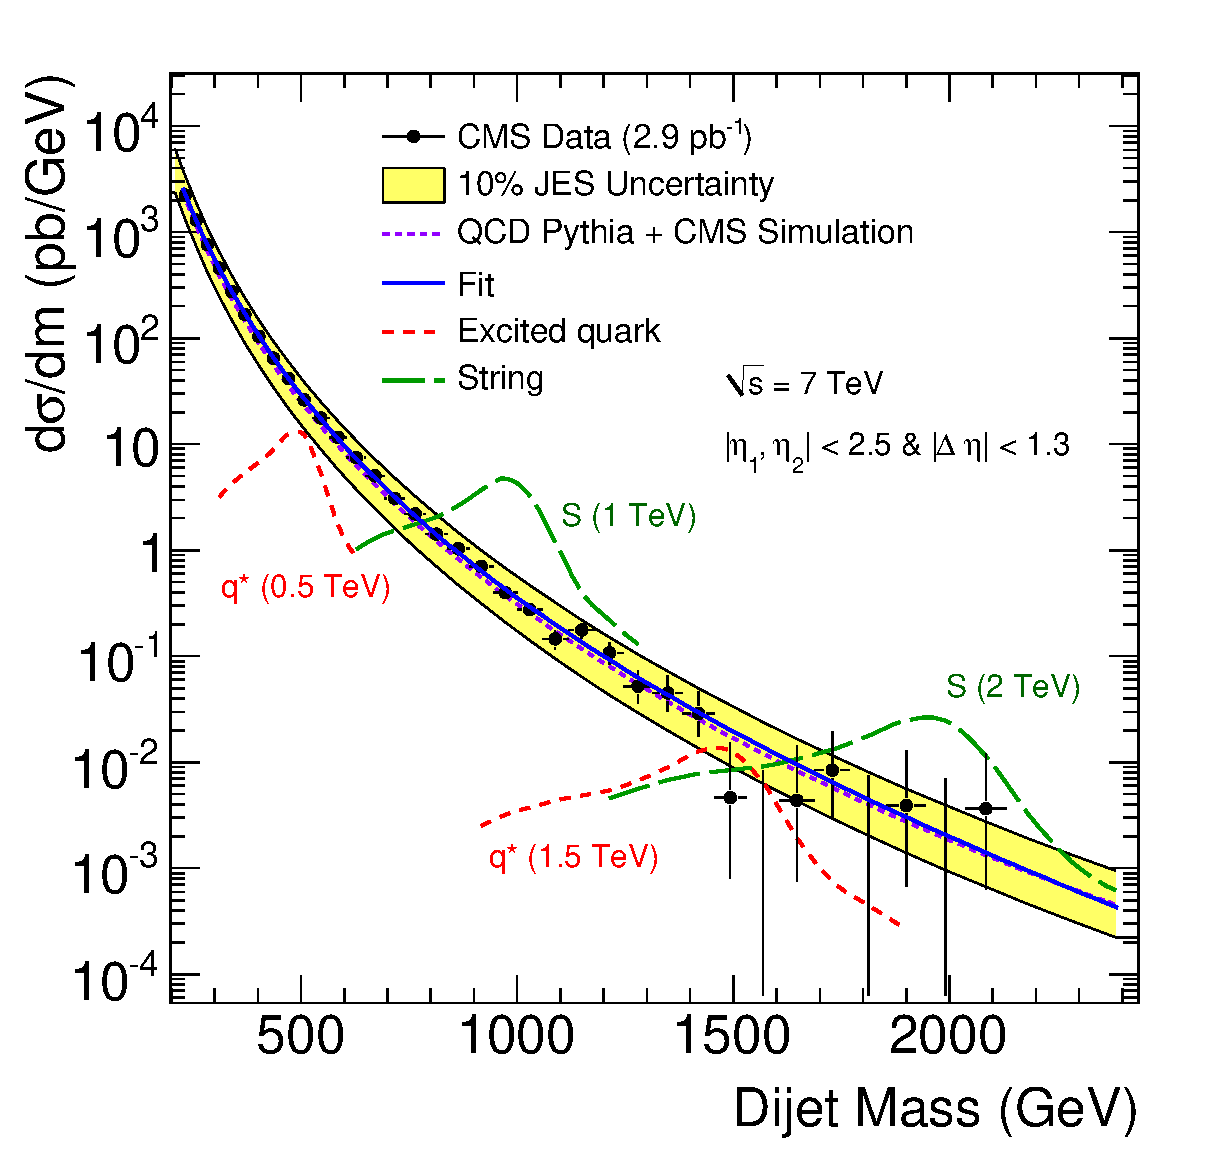
\includegraphics[width=1.0\textwidth]{DijetMassFit}
    \hspace{1cm}
    \caption{
   Measured cross section (points) as a function of the dijet mass compared to a smooth fit (solid blue) 
    and to simulations~\cite{refPYTHIA} of QCD (dashed blue), excited quark signals (dashed red), 
    and string resonance signals (dashed green) in the CMS detector.
     The yellow band shows the sensitivity to a 10\% systematic uncertainty on the jet energy scale.}
    \label{fig1}
  \end{center}
\end{figure}


\begin{figure}[hbtp]
  \begin{center}
    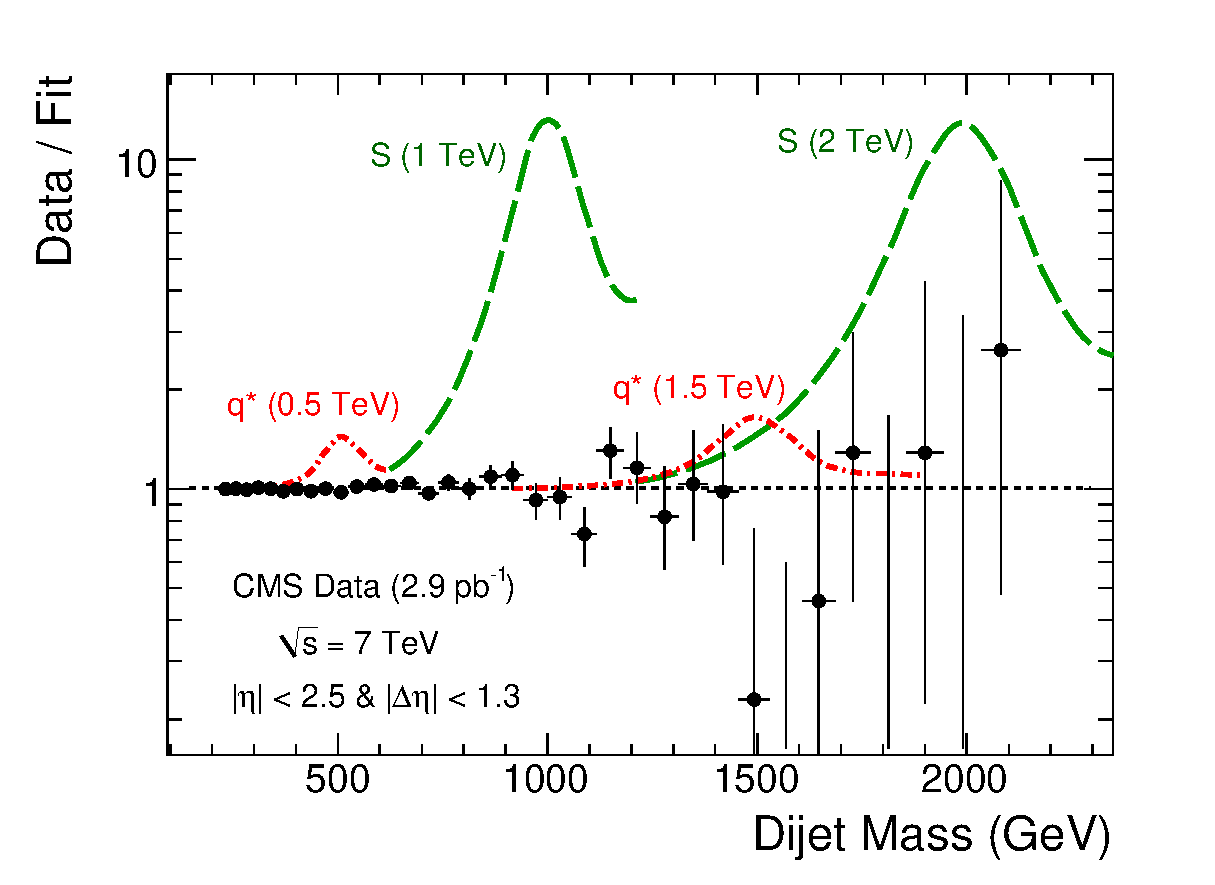
\includegraphics[width=1.0\textwidth]{DijetDataOverFit}
    \hspace{1cm}
    \caption{The ratio between the dijet mass data (points) and a smooth
background fit (dashed line) is compared to simulations of excited quark signals 
(dot-dashed red curves) and string resonance signals (dashed green curves).}
    \label{fig2}
  \end{center}
\end{figure}


\begin{figure}[hbtp]
  \begin{center}
    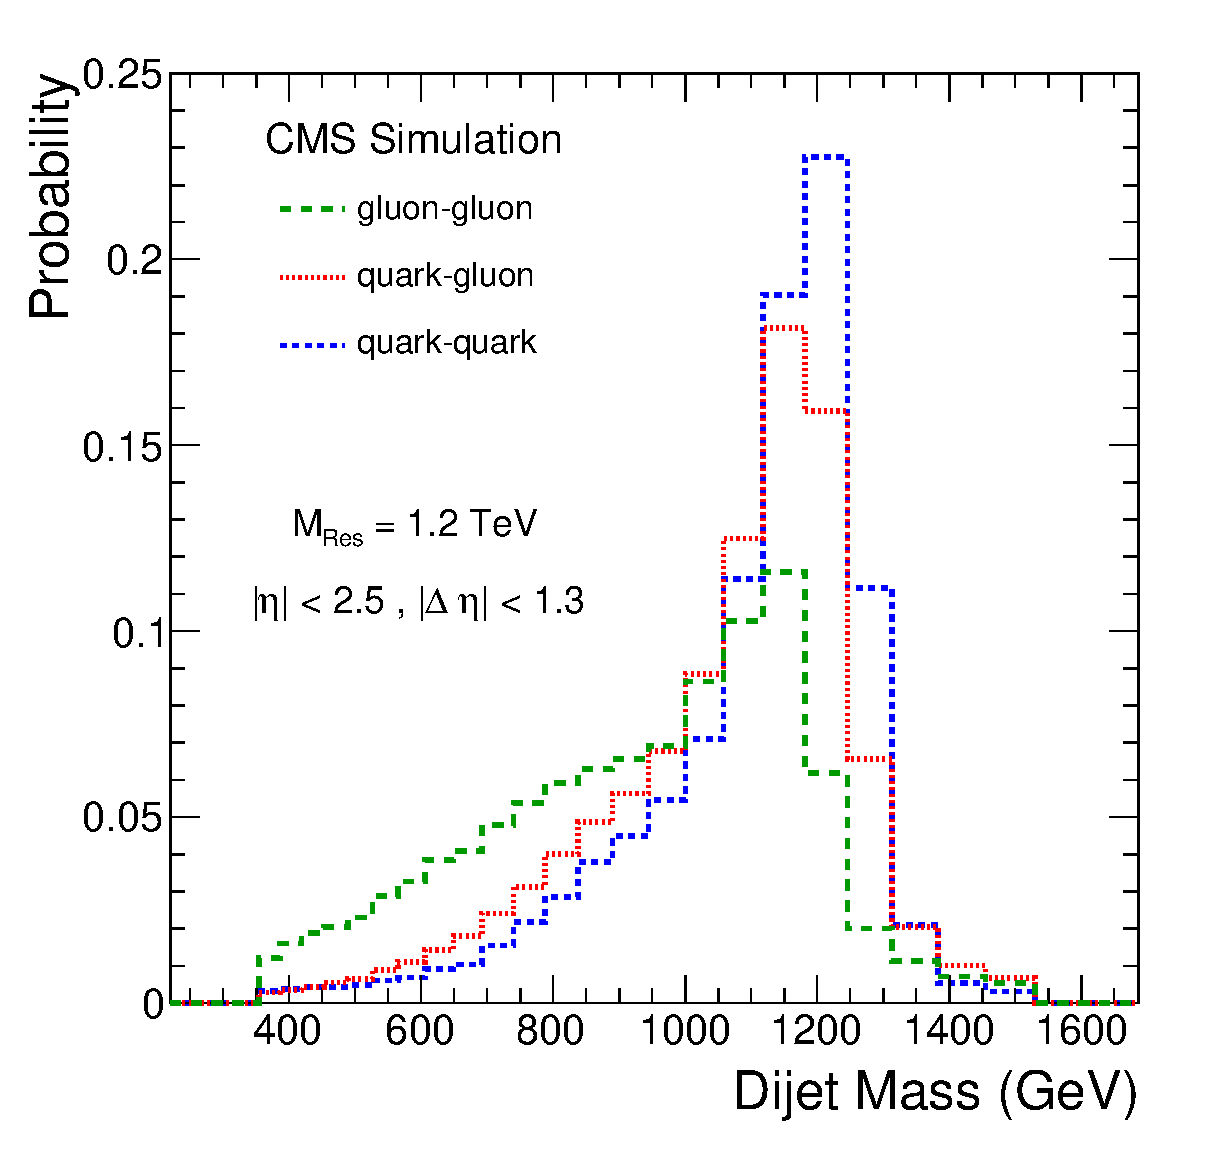
\includegraphics[width=1.0\textwidth]{DijetResonanceTypes}
    \hspace{1cm}
    \caption{Simulations of the dijet mass distribution for narrow resonances 
with the mass of 1.2 TeV involving parton pairs of type quark-quark (blue), quark-gluon (red), 
and gluon-gluon (green).}
    \label{fig3}
  \end{center}
\end{figure}


\begin{figure}[hbtp]
  \begin{center}
    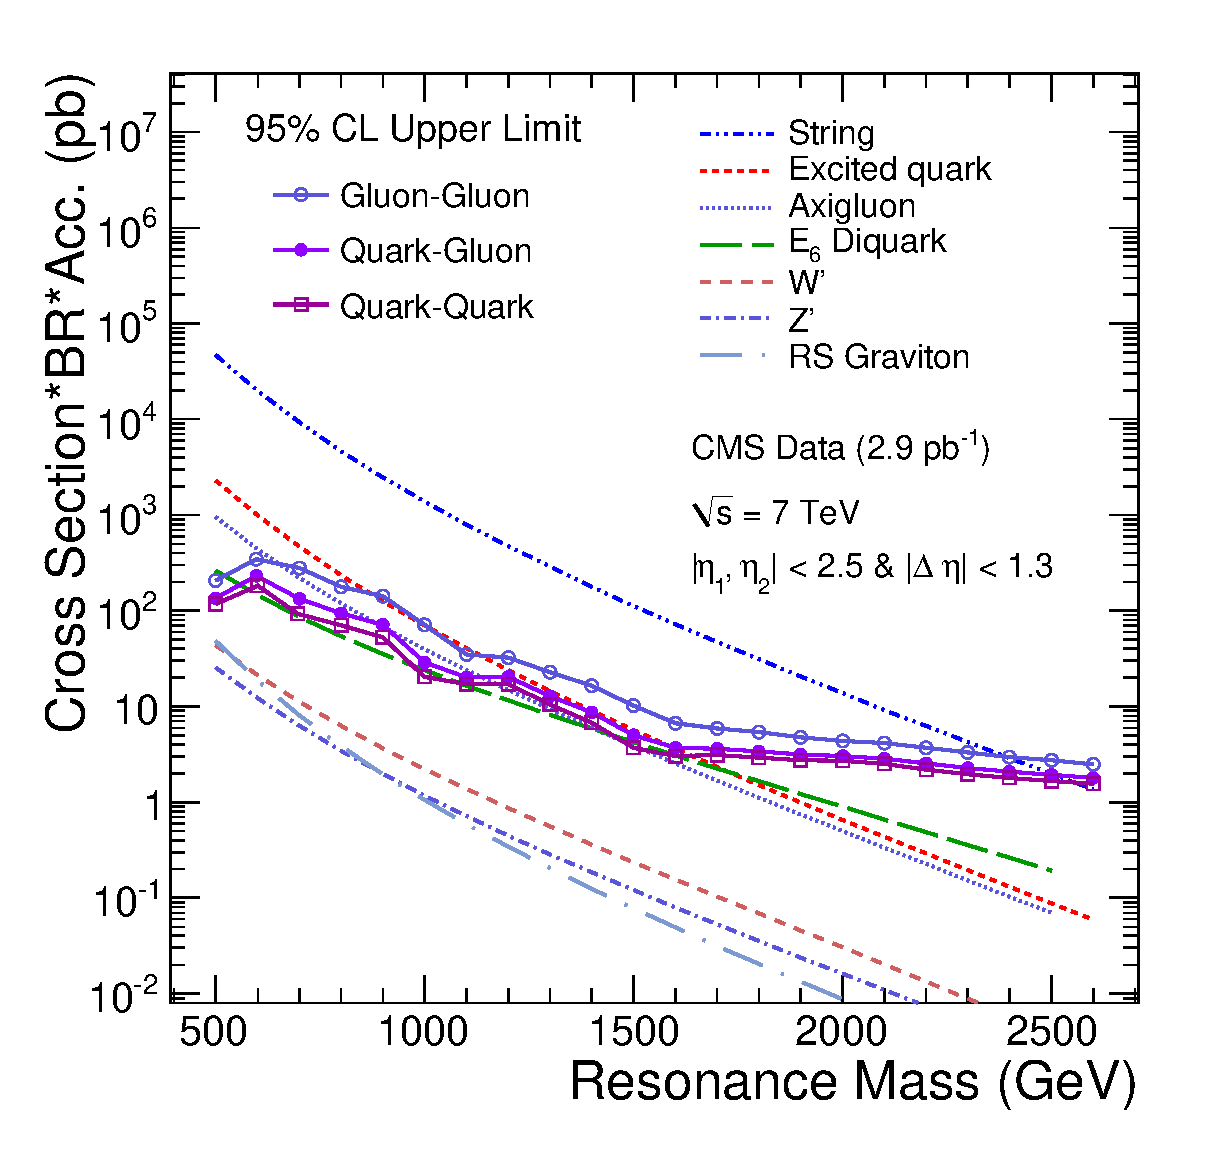
\includegraphics[width=1.0\textwidth]{DijetLimit}
    \hspace{1cm}
    \caption{95\% CL upper limits on the cross section times branching 
fraction times acceptance for dijet resonances of type gluon-gluon 
(open circles), quark-gluon (solid circles), and quark-quark (open boxes) 
compared to 
theoretical predictions for string resonances~\cite{Anchordoqui:2008di}, excited
quarks~\cite{ref_qstar}, axigluons~\cite{ref_axi}, 
colorons~\cite{ref_coloron}, $E_6$ diquarks~\cite{ref_diquark}, Randall-Sundrum
gravitons~\cite{ref_rsg}, and 
new gauge bosons $W^{\prime}$ and $Z^{\prime}$~\cite{ref_gauge}.}
    \label{fig4}
  \end{center}
\end{figure}


\begin{table}[htbH]
\begin{center}
\caption{
Upper limits at 95\% C.L.on cross section times branching fraction times acceptance, 
listed as a function of new particle mass, for narrow resonances decaying to dijets 
with partons of type quark-quark ($qq$), quark-gluon ($qg$), and gluon-gluon ($gg$).
The limits apply to the kinematic range where both jets have pseudorapidity 
$|\eta|<2.5$ and $|\Delta\eta|<1.3$.
}
\label{tab_limit}
\vspace*{1cm}
\begin{tabular}{|c|c|c|c|}\hline 
Mass   &  \multicolumn{3}{c|}{Limit (pb)}\\
 (TeV) &  qq & qg & gg\\ \hline
0.5	 &  118	         &  134	         &  206  \\  
0.6	 &  182	         &  229	         &  339  \\  
0.7	 &  90.7         &  134	         &  281  \\  
0.8	 &  70.8	 &  93.5	 &  177  \\  
0.9	 &  52.7	 &  71.6	 &  142  \\  
1.0	 &  20.3	 &  29.0	 &  71.4 \\  
1.1	 &  17.0	 &  20.1	 &  35.1 \\  
1.2	 &  17.0	 &  20.4	 &  32.5 \\  
1.3	 &  10.5	 &  12.9	 &  22.8 \\  
1.4	 &  6.77	 &  8.71	 &  16.4 \\  
1.5	 &  3.71	 &  5.02	 &  10.3 \\  
1.6	 &  3.05	 &  3.72	 &  6.71 \\  
1.7	 &  3.13	 &  3.64	 &  5.88 \\  
1.8	 &  2.92	 &  3.41	 &  5.37 \\  
1.9	 &  2.73	 &  3.15	 &  4.78 \\  
2.0	 &  2.71	 &  3.02	 &  4.39 \\  
2.1	 &  2.50	 &  2.84	 &  4.15 \\  
2.2	 &  2.20	 &  2.55	 &  3.69 \\  
2.3	 &  1.96	 &  2.28	 &  3.32 \\  
2.4	 &  1.79	 &  2.08	 &  2.94 \\  
2.5	 &  1.67	 &  1.93	 &  2.74 \\
2.6	 &  1.55	 &  1.80	 &  2.50 \\
\hline
\end{tabular}
\end{center}
\end{table}

